\id{ҒТАМР 06.52.41}{}

\begin{articleheader}
\sectionwithauthors{Ж.Д.Серикбаева, К.А.Мадыханова, А.С.Бактымбет}{ЛАТЫН АМЕРИКАСЫ ЕЛДЕРІНДЕГІ ӨНЕРКӘСІПТІК САЯСАТ}

{\bfseries
\textsuperscript{1}Ж.Д.Серикбаева,
\textsuperscript{2}К.А.Мадыханова\textsuperscript{\envelope },
\textsuperscript{3}А.С.Бактымбет
}
\end{articleheader}

\begin{affiliation}
\textsuperscript{1,2}Алматы Менеджмент Университеті, Алматы, Қазақстан,

\textsuperscript{3}Т. Құлажанов атындағы Қазақ технология және бизнес университеті, Астана, Қазақстан

\raggedright \textsuperscript{\envelope }Корреспондент-автор: madyxanova77@mail.ru
\end{affiliation}

Бұл мақала Латын Америкасы елдерінің индустриялық саясатының құрылымын,
мәселелерін және перспективаларын талдауға арналған. Өңірдегі негізгі
экономикалық және құрылымдық өзгерістер, жаһандық экономикалық
процестердің әсері және өнеркәсіптің ішкі даму динамикасы зерттеледі.
Мақалада шикізат экспортына тәуелділік, жаһандық құн тізбектеріне төмен
қатысу және инновацияларға шектеулі инвестициялар сияқты
макроэкономикалық қиындықтар қарастырылады. Чили, Бразилия және Мексика
сияқты елдердің табысты өнеркәсіптік стратегияларын қолдану тәжірибесі
талданады. Зерттеуде экономикалық, тарихи және саяси талдауды қамтитын
пәнаралық әдіс, сондай-ақ қаржылық құжаттар мен стратегияларды
контент-талдау қолданылды. Мексикадағы автомобиль өнеркәсібі және
Бразилиядағы авиация саласы сияқты кластерлік бастамалардың мысалдары
қарастырылған. Өнеркәсіптік саясаттың табысты болуына әсер ететін
факторларға ерекше назар аударылады, соның ішінде ұзақ мерзімді
жоспарлау, жеке сектордың қатысуы, ішкі сұранысты дамыту және іске асыру
механизмдерінің икемділігі. Өңірдің ерекшеліктерін ескере отырып,
халықаралық тәжірибені бейімдеудің, мемлекеттің және жеке сектордың
тұрақты индустриялық саясатты қалыптастыруға белсенді қатысуының
маңыздылығы туралы қорытынды жасалды.

{\bfseries Түйін сөздер}: индустриялық саясат, Латын Америкасы,
экономикалық даму, инновациялар, макроэкономика, жаһандық құн
тізбектері, инвестициялар, кластерлік бастамалар.

\begin{articleheader}
{\bfseries ИНДУСТРИАЛЬНАЯ ПОЛИТИКА В СТРАНАХ ЛАТИНСКОЙ АМЕРИКИ}

{\bfseries
\textsuperscript{1}Ж.Д.Серикбаева,
\textsuperscript{2}К.А.Мадыханова\textsuperscript{\envelope },
\textsuperscript{3}А.С.Бактымбет
}
\end{articleheader}

\begin{affiliation}
\textsuperscript{1,2}Алматы Менеджмент Университет, Алматы, Казахстан,

\textsuperscript{3}Казахский университет технологии и бизнеса им. К. Кулажанова, Астана, Казахстан,

e-mail: madyxanova77@mail.ru
\end{affiliation}

Статья посвящена анализу индустриальной политики стран Латинской
Америки, ее структуре, проблемам и перспективам. Исследуются ключевые
экономические и структурные изменения в регионе, влияние глобальных
экономических процессов и внутренняя динамика развития промышленности. В
работе рассматриваются макроэкономические вызовы, включая зависимость от
экспорта сырья, низкий уровень участия в глобальных цепочках добавленной
стоимости и ограниченные инвестиции в инновации. Анализируется опыт
различных стран региона, включая Чили, Бразилию и Мексику, в применении
успешных промышленных стратегий. В статье использован междисциплинарный
подход, включающий экономический, исторический и политический анализ, а
также контент-анализ финансовых документов и стратегий. Рассмотрены
примеры кластерных инициатив, таких как автомобильная промышленность
Мексики и авиационная отрасль Бразилии. Особое внимание уделено
факторам, влияющим на успех промышленной политики, включая долгосрочное
планирование, участие частного сектора, развитие внутреннего спроса и
гибкость механизмов реализации. Сделан вывод о необходимости адаптации
международного опыта к специфике региона, активного вовлечения
государства и частного сектора в формирование устойчивой индустриальной
политики.

{\bfseries Ключевые слова:} индустриальная политика, Латинская Америка,
экономическое развитие, инновации, макроэкономика, глобальные цепочки
добавленной стоимости, инвестиции, кластерные инициативы.

\begin{articleheader}
{\bfseries INDUSTRIAL POLICY IN LATIN AMERICAN COUNTRIES}

{\bfseries
\textsuperscript{1}Zh.D.Serikbaeva,
\textsuperscript{2}K.A.Madykhanova\textsuperscript{\envelope },
\textsuperscript{3}A.S.Baktymbet
}
\end{articleheader}

\begin{affiliation}
\textsuperscript{1,2}Almaty Management University, Almaty, Kazakhstan,

\textsuperscript{3}Kazakh University of Technology and Business named after K. Kulazhanov, Astana, Kazakhstan,

e-mail: madyxanova77@mail.ru
\end{affiliation}

This article analyzes the industrial policy of Latin American countries,
its structure, challenges, and prospects. It examines key economic and
structural changes in the region, the impact of global economic
processes, and the internal dynamics of industrial development. The
study addresses macroeconomic challenges such as dependence on raw
material exports, low participation in global value chains, and limited
investments in innovation. The experience of countries like Chile,
Brazil, and Mexico in implementing successful industrial strategies is
analyzed. The research employs an interdisciplinary approach that
includes economic, historical, and political analysis, as well as
content analysis of financial documents and strategies. Examples of
cluster initiatives, such as Mexico's automotive industry and Brazil's
aviation sector, are considered. Special attention is given to factors
influencing the success of industrial policy, including long-term
planning, private sector involvement, domestic demand development, and
flexibility in implementation mechanisms. The article concludes that
adapting international experience to regional specifics and ensuring
active participation of both the state and the private sector are
crucial for the development of a sustainable industrial policy.

{\bfseries Keywords:} industrial policy, Latin America, economic
development, innovation, macroeconomics, global value chains,
investments, cluster initiatives.

\begin{multicols}{2}
{\bfseries Кіріспе.} Соңғы екі онжылдықта жаһандық экономикалық жағдай
айтарлықтай өзгерістерге ұшырады. Қытай экономикасының өсуі, геосаяси
өзгерістер және цифрлық революция тез өзгеретін экономикалық ландшафтты
қалыптастыруда. Оңтүстік-Шығыс Азия мен Тынық мұхиты аймағы өзінің өсіп
келе жатқан жаһандық маңыздылығымен назар аударады. Африка халқының
қарқынды өсуімен және аймақ басшыларының жаңа даму стратегиясын
қалыптастыруымен ерекшеленеді. Ал Латын Америкасы мен Кариб бассейні
елдерінің даму перспективалары әлі де күрделі күйде қалып отыр.2023
жылы экономикалық өсім тұрақты тұтыну мен инвестициялардың, капитал
ағынының және сыртқы сұраныстың арқасында күткеннен жоғары болды.
Дегенмен, инфляция төмендегенімен, ол әлі де жоғары деңгейде сақталуда,
ал құрылымдық қиындықтар мен макроэкономикалық саясат мәселелері
өзектілігін жоғалтқан жоқ.2024 жылы қаржылық жағдайдың қатаңдауы ішкі
сұранысқа әсер етіп, Қытай мен АҚШ-тағы экономикалық өсімнің баяулауы
экспортты тежеді {[}1{]}.

Кедейлік деңгейінің төмендеуі, табыстардың бөлінуінің жақсаруы, білім
беру мен денсаулық сақтау салаларына қолжетімділіктің артуы және
цифрландырудағы жетістіктерге қарамастан, Латын Америкасы елдері әлі де
экономикалық тұрақсыздықпен сипатталады. Негізгі мәселе - бұл аймақ
әлемдік нарықта шикізат жеткізуші мәртебесінен шығып, жаһандық құн
тізбектеріне қалай тиімдірек қатыса алады деген сұрақта. Бұл қатысудың
артуы жергілікті экономикалық субъектілер үшін тиімді болуы керек
{[}2{]}.

Бұл мақалада Латын Америкасы елдеріндегі өнеркәсіптік саясатты жүзеге
асыру мәселелері қарастырылады. Бұл аймақ біртектіліктен алыс: елдер
экономикалық дамудың әртүрлі деңгейінде және нарық көлемі әртүрлі.
Дегенмен, бұл елдердің ортақ тарихи-мәдени мұрасы және индустриялық
саясатты жүзеге асырудағы ортақ көзқарастары бар. Латын Америкасы
елдерінің тәжірибесі, макроэкономикалық саясаттың проблемаларына
қарамастан, бай және елдер таныс технологияларды қалай және неге
толығымен өзгертетіні және кадрларды қайта дайындайтыны, неге
кейбіреулер басқаларға қарағанда тезірек және жақсырақ үйренеді және
неге кейбіреулері өнеркәсіптік саясатты дамыту үшін қажетті тетіктерді
іске қоспай жатқаны туралы қызықты сабақтар ұсынады.

Біз бірнеше Латын Америкасы елдерінің тәжірибесін қарастырамыз және ең
дамыған және өнеркәсібі дамыған елдерге назар аударамыз. Біз мақаланы
Латын Америкасындағы экономикалық даму және құрылымдық өзгерістер туралы
статистикалық мәліметтерге талдау жасаудан, аймақ елдеріндегі
өнеркәсіптік даму проблемаларын, өндіріс пен сауданың басым үлгілерінен
туындайтын білім беру жүйесінің кемшіліктерін, білім базасының
шектеулілігін қарастырудан бастаймыз. Содан кейін ол Латын Америкасының
өнеркәсіптік саясатындағы жаңа мүмкіндіктер мен инновациялық тәсілдерді
талдайды. Мақаланың соңында Латын Америкасындағы табысты өнеркәсіптік
саясат мысалдарына назар аударылады. Мақалада өнеркәсіптік саясатты
дамытудың әмбебап тәсілі жоқ, бірақ экономикалық дамудың қолайлы
тетіктерін іске қосатын жалпы принциптер бар деп қорытындыланады.

Өндіріс жүйелерінің жаһандық трансформациясы және ресурстар мен нарықтар
үшін бәсекелестіктің күшеюі жағдайында өнеркәсіптік саясат экономикалық
даму стратегиясында тағы да басты мәнге ие болуда.
Әлеуметтік-экономикалық, саяси және институционалдық факторлардың
тоғысында индустриялық стратегиялар қалыптасатын Латын Америкасы
елдерінің тәжірибесіне ерекше назар аударылады. Осы макроөңірдегі
өнеркәсіптік саясатты талдау дамудың экономикалық теорияларының ықпалын,
саяси-құқықтық реттеу тетіктерін, сондай-ақ аймақтың тарихи-мәдени
ерекшеліктерін жан-жақты қарастыруға мүмкіндік беретін пәнаралық
көзқарасты қажет етеді. Экономиканың, саясаттанудың, институционалдық
теорияның және аймақтанудың әдістері мен концептуалды негіздерін
біріктіру Латын Америкасы елдерінде олардың құрылымдық шектеулерін,
әлеуметтік біркелкі еместігін және әлемдік үрдістерге тәуелділігін
ескере отырып, индустриялық стратегияларды қалыптастыру және жүзеге
асыру заңдылықтарын неғұрлым толық ашуға мүмкіндік береді.

{\bfseries Материалдар мен әдістер.} Бұл зерттеу барысында Латын Америкасы
елдерінің индустриялық саясатын кешенді талдауға мүмкіндік беретін түрлі
әдістер қолданылды. Негізгі назар экономикалық, тарихи және саяси
талдауды қамтитын пәнаралық әдіске аударылды.

1. Ғылыми әдебиеттерді талдау. UNCTAD, ABDI, ECLAC/CEPAL сияқты
халықаралық ұйымдардың жарияланымдары мен Латын Америкасы елдерінің
индустриялық саясатына арналған академиялық жұмыстар зерттелді.

2. Қаржылық құжаттар мен стратегиялық жоспарларды контент-талдау.
Үкіметтік құжаттар, стратегиялық жоспарлар, заңнамалық актілер мен
экономикалық даму бағдарламалары талданды.

3. Кросс-мәдени талдау. Латын Америкасы елдерінің ортақ тарихи негіздері
болғанымен, олардың экономикалық даму модельдері әртүрлі. Бұл зерттеу
жалпы заңдылықтар мен әр елге тән ерекшеліктерді анықтауға көмектесті.

4. Кластерлік бастамаларды талдау. Латын Америкасының өнеркәсіптік
саясатындағы табысты кластерлік стратегиялардың үлгілері, мысалы,
Мексикадағы автомобиль кластерлері мен Бразилиядағы авиация
индустриясы зерттелді.

{\bfseries Нәтижелер және талқылау.} Латын Америкасы дамуының баяу
қарқынымен ерекшеленетін әлемдік экономикалық жағдай жоғары жылдамдықпен
өзгеруде. Латын Америкасының жаһандық ЖІӨ-ге қосқан үлесі 1960 жылдардан
бері шамамен 7,5\% деңгейінде тұрақты болды (сурет 1) {[}3{]}.
Оңтүстік-Шығыс Азия мен Тынық мұхиты аймағының көтерілуі, атап айтқанда,
1970 жылдардың соңынан бастап Қытайдың жедел көтерілуі жаһандық
экономика эволюциясының маңызды кезеңі болды {[}4{]}. Оңтүстік-Шығыс
Азия мен Тынық мұхиты елдері қазір жаһандық ЖІӨ-нің 28\% құрайды, бұл
1960 жылғы 12\% -дан жоғары және 2007 жылдан бері әлемдегі жетекші
экономика ретінде АҚШ-ты басып озды {[}5{]}.

Алайда 2014 жылы Латын Америкасы елдерінің әлемдік ЖІӨ-дегі үлесі
7,9\%-ды құраса, 2021 жылы бұл көрсеткіш шамамен 2\%-ға төмендеді
{[}6{]}.

Қытай шамамен отыз жыл бойы жаһандық экономикалық өсудің негізгі
драйвері болды.1990 және 2020 жылдар аралығында бұл ел әлемдік ЖІӨ
өсімінің төрттен бірінен астамын құрады.2013 және 2021 жылдар
аралығында Қытай жаһандық ЖІӨ өсімінің 39\%-ға жуығын құрады, бұл G7
елдерін біріктіргеннен 13\%-ға көп {[}7{]}.

Халықаралық валюта қорының (ХВҚ) мәліметі бойынша Қытай қазіргі уақытта
номиналды ЖІӨ көлемі бойынша әлемде екінші орында тұр. Азияның басқа
экономикалары да ең үлкендердің қатарында, Жапония ЖІӨ бойынша әлемде
төртінші, ал Үндістан бесінші орында.
\end{multicols}

\begin{figure}[H]
	\centering
	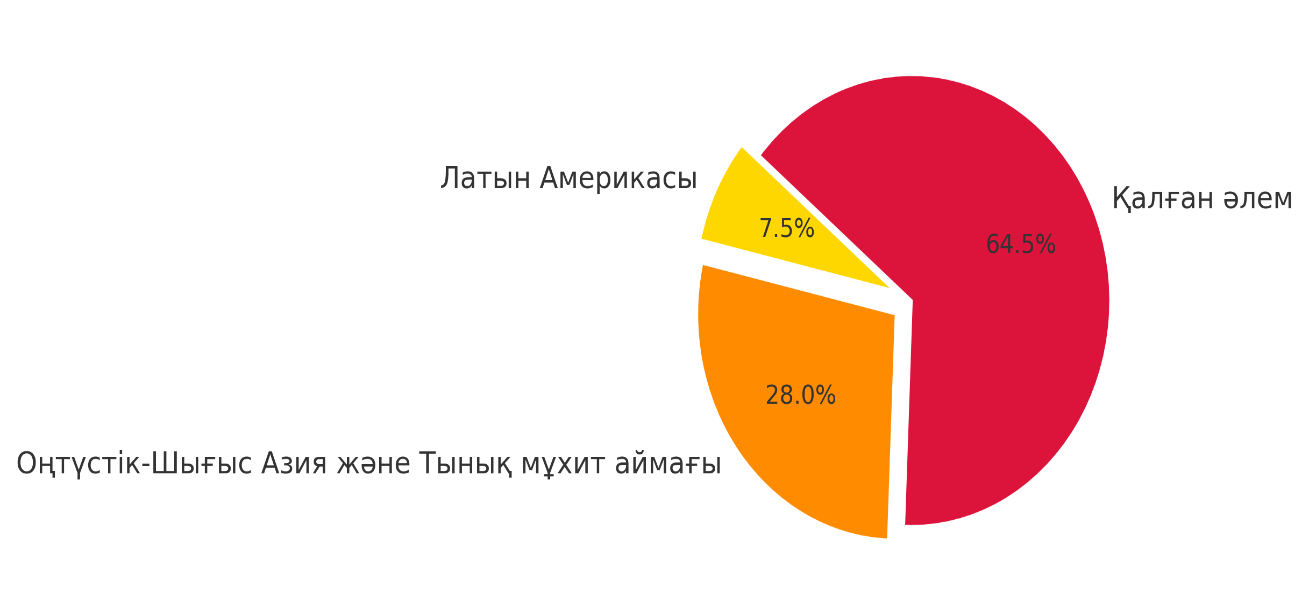
\includegraphics[width=0.8\textwidth]{media/ekon2/image51}
	\caption*{1 - сурет. Латын Америкасының әлемдік ЖІӨ-дегі үлесі}
\end{figure}

\begin{multicols}{2}
Жапония бұған дейін әлемдегі үшінші ірі экономика болды, бірақ ол 2023
жылдың үшінші және төртінші тоқсанында ІЖӨ-нің қысқаруы нәтижесінде
техникалық рецессияға түсіп, Германияға бұл позициясын ұсынды {[}8{]}.

Латын Америкасы экономикалық динамизмнің аздығымен сипатталады.
Африкадан, Қытайдан және Оңтүстік-Шығыс Азиядан айырмашылығы, аймақ ұзақ
мерзімді кезеңде орташа әлемдік деңгейден баяу өсті. Тауарларға
сұраныстың өсуіне және ішкі сұраныс арқылы ЖІӨ өсуін қамтамасыз ете
алатын өсіп келе жатқан орта тапқа қарамастан, аймақ осы кезеңді
сипаттайтын экономикалық өсу қарқынын қалпына келтіруден алыс. Соңғы
онжылдықтағы аймақтың ЖІӨ-нің орташа өсімі ел әлемдік нарықта бәсекеге
қабілетті отандық өнеркәсіптік әлеуетті құруға бағытталған мемлекеттік
даму және импортты алмастыру саясаты кезеңінде болған 1950 және 1960
жылдардағы көрсеткіштің жартысын ғана құрайды (сурет 2).
\end{multicols}

\begin{figure}[H]
	\centering
	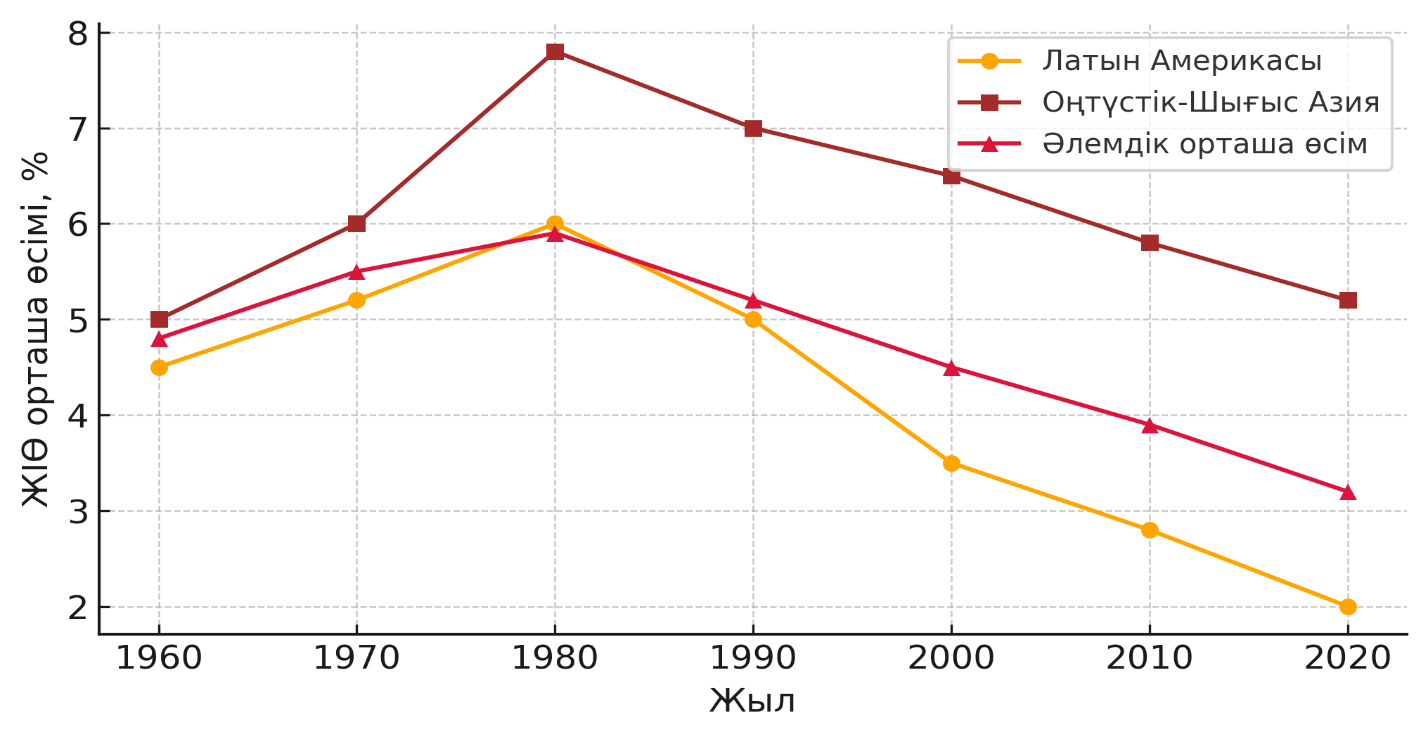
\includegraphics[width=0.8\textwidth]{media/ekon2/image52}
	\caption*{2 - сурет. Латын Америкасы және басқа аймақтардағы ЖІӨ өсу динамикасы}
\end{figure}

\begin{multicols}{2}
Өнеркәсібі дамыған елдердің тәжірибесін пайдалану дамушы елдердің алға
жылжуына мүмкіндік береді, ол шын мәнінде ЖІӨ мен өнімділіктің өсу көзі
болып табылады {[}9{]}. Тәжірибемен алмасу әртүрлі деңгейде өтеді. Бір
жағынан, ол саясат пен институционалдық даму деңгейінде жүзеге
асырылады; екінші жағынан, өндіріс процесінде және инновациялық
жүйелерде әртүрлі деңгейлерде орын алады: секторлар мен құн тізбегінде,
фирмаларда, аумақтық кластерлерде және жеке деңгейде. Азиямен
салыстырғанда Латын Америкасының шектеулі экономикалық өсу көрсеткіштері
оның жаһандық экономикаға маргиналды, біркелкі интеграциялануымен,
аймақтың тұрақты құрылымдық инерциясымен және осыған байланысты оқу
мүмкіндіктерінің шектелуімен байланысты {[}10{]}. Бір жағынан, Латын
Америкасы тауарлармен байланысты болып қала береді және жаһандық құн
тізбегіне шектеулі қатысуға ие. Экономикалық күрделіліктің
Хидалго-Хаусман индексі соңғы екі онжылдықта азиялық табыстар тарихында
көтерілгенімен, Оңтүстік Америкада, Орталық Америкада және Кариб
бассейнінде өте төмен болып қалды. Өңірдегі елдер ресурстарды көп қажет
ететін қызметке немесе жаһандық құн тізбегіндегі құрастыру желілеріне
маманданған жоқ, сонымен бірге олардың көпшілігі өнеркәсіптік
мүмкіндіктеріне зиян келтіре отырып, уақыт өте келе табиғи ресурстарға
тәуелділігін арттырды. Мысалы, Чилиде тау-кен экспортының жалпы
экспорттағы үлесі 1990 жылдан 2017 жылға дейін 40\%-дан 50\%-ға дейін
өссе, Колумбияда мұнай экспортының үлесі 25\%-дан 50\%-ға дейін өсті
{[}11{]}.

Латын Америкасында құрылымдық өзгерістерге және экономиканы
әртараптандыруға қол жеткізу өнеркәсіптік саясаттың негізгі мақсаты
болып қала береді. Өңдеу өнеркәсібі -- облыстың материалдық өндірісінің
негізгі саласы. Мұнда Латын Америкасының экономикалық белсенді халқының
шамамен 15\% жұмыс істейді.1960 жылдардың соңына дейін өңдеу
өнеркәсібінің жетекші саласы тамақ өнеркәсібі болды, ал 1970 жылдардан
бастап оны металл өңдеу және машина жасау басып озды. Дегенмен, Латын
Америкасының өңдеу өнеркәсібі қазір Қытайдың бәсекелестігінің күшеюіне
және ғылыми зерттеулер мен инновацияларға инвестицияның шектеулі болуына
байланысты өз орнын жоғалтып жатыр.
\end{multicols}

\begin{figure}[H]
	\centering
	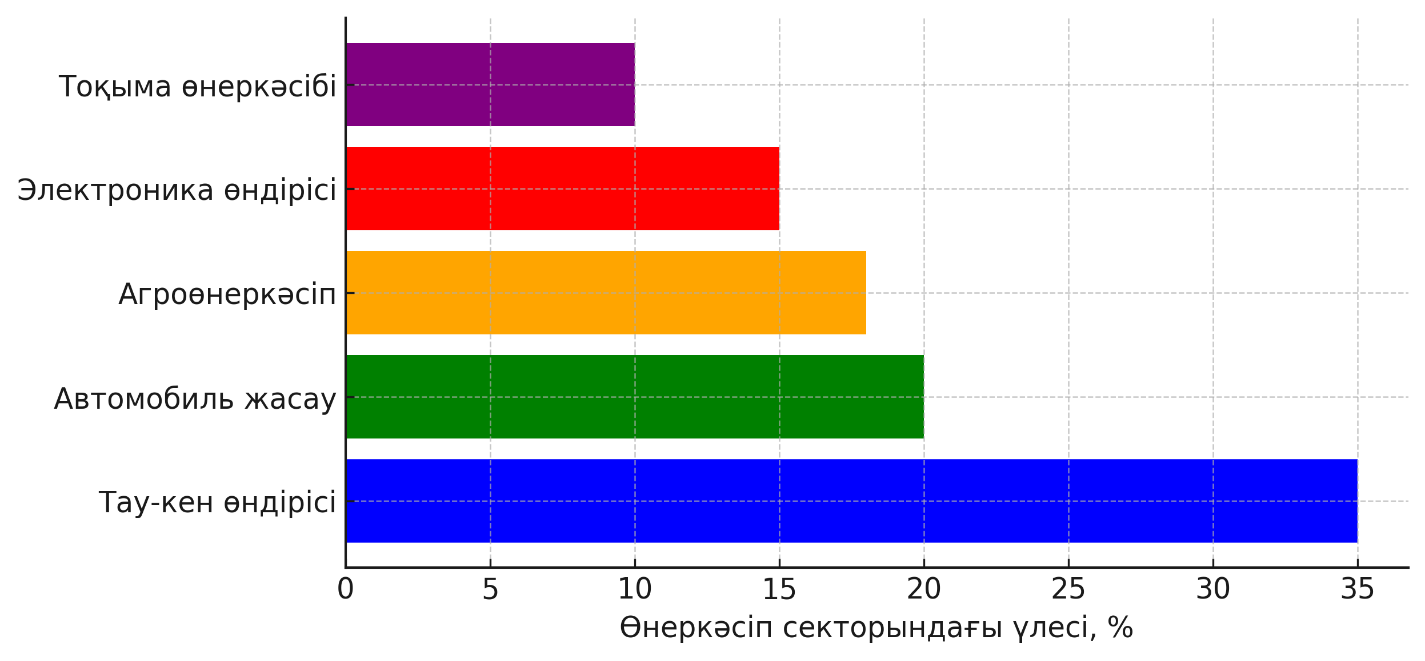
\includegraphics[width=0.8\textwidth]{media/ekon2/image53}
	\caption*{3 - сурет. Латын Америкасындағы негізгі өнеркәсіптер, 2023ж. {[}8{]}}
\end{figure}

\begin{multicols}{2}
Өңірдегі экономикалардың көпшілігі төмен өнімділік және экономикалық
құрылымдарының жеткіліксіз әртараптандыру проблемаларымен бетпе-бет
келеді. Бұл сипаттамалар мүмкіндіктердің бірнеше фирмаларда, секторларда
және аумақтарда шоғырлануымен байланысты. Мысалы, Чилиде ірі фирмалар
экономикада басым рөл атқарады, бірақ олар дамыған елдердегі
әріптестеріне қарағанда жаңашылдығы төмен. Чилидегі ірі фирмалар бизнес
айналымының 73\% және жалпы ҒЗТКЖ-ның 57\% құрайды, ал Германияда мұндай
фирмалар айналымның 53\% және ҒЗТКЖ-ның 85\% құрайды {[}11{]}.

Өнеркәсіптік саясат (әртүрлі формада және әртүрлі атаулармен) 1950
жылдардан бері Латын Америкасы үшін жаңалық емес {[}12{]}. Алайда,
1950-1970 жылдар аралығын қоспағанда, олар ұлттық даму стратегияларында
маңызды рөл атқара алмады. Олардың дамуы жүйелі болған жоқ және олар
қайтадан ұлттық даму стратегияларының бір бөлігіне айналса да, Латын
Америкасын жаңғыртудың бастапқы кезеңіне тән амбиция мен инвестицияны
ешқашан қайтара алмады {[}11{]}.

1980-1990 жылдар аралығында бірте-бірте индустрияландыруға, біліктілікті
арттыруға және өндірістік мүмкіндіктерді жинақтауға бағытталған
өнеркәсіп саясаты бұрынғы танымалдылығын жоғалтып, экономикалық дамудың
онша маңызды емес стратегиясына айналды. Іс жүзінде ырықтандыру
кезеңінде өнеркәсіптік саясаттың кейбір құралдары белсенді болғанымен,
олар бәсекеге қабілеттілік және кластерді дамыту саясаты сияқты нарыққа
қолайлы тұжырымдамалар ретінде ұсынылды {[}13{]}. Сол кезде аймақтағы
өнеркәсіптік саясатқа қатысты басым пікірді «Ең жақсы өнеркәсіптік
саясат -- өнеркәсіптік саясат жоқ» деген атақты сөз тіркесімен
түйіндеуге болады {[}14{]}. Ресурстарды бөлу және ынталандыру механизмі
ретінде нарықтың артықшылығына идеологиялық сенім мемлекеттің
экономикаға белсенді араласуының қауіптілігі туралы кең алаңдаушылықты
тудырды және сыбайлас жемқорлық пен билікті басып алу тәуекелдерін
барынша азайту мақсатында даму стратегияларына ұстамды көзқарасты
ынталандырды. Содан бері өнеркәсіптік саясаттар аймаққа әртүрлі
нысандарда және вариацияларда қайта оралды, бірақ олардың әсері, бірнеше
оқшауланған сәтті жағдайларды қоспағанда, күткеннен төмен болды.

Латын Америкасында өнеркәсіптік саясаттың әлсіз болуының көптеген
себептері бар. Олардың ішінде ең маңыздысы басқа аймақтардағы
өнеркәсіптік саясат табысының әртүрлі факторларының Латын Америкасының
тәжірибесінде жоқтығымен байланысты. Латын Америкасындағы өнеркәсіпті
дамыту саясаты әрқашан Оңтүстік-Шығыс Азия елдерінің экспортқа
бағытталған өршіл индустрияландыру стратегияларынан, тіпті одан әрі
отандық өнеркәсіпке басымдық берудің бүкіл үкіметтік көзқарасынан және
АҚШ-та әрқашан басым болған технологиялар мен зерттеулерге баса назар
аударудан алыс болды. Оның үстіне олар экономикасы табысты елдердегідей
дәйектілікпен және бюджеттік қолдаумен жүзеге асырылмайды.

Латын Америкасындағы өнеркәсіптік даму саясатының бастамалары
инновацияларды дамыту мен енгізуге және елдердің технологиялық
алшақтығын еңсеруге қатысты баламалы ойлау мен перспективаларды
қалыптастыруға бағытталған. Салық жеңілдіктерін беруге, ҒЗТКЖ және
инновациялық қызметтің басқа да түрлеріне жұмсалатын шығындарды
арттыруға баса назар аударылды. Саясатты әзірлеуде оқыту екі негізгі
арна арқылы жүзеге асады: орындау арқылы үйрену (яғни, тәжірибе жасау
және жаңа саясаттарды енгізу арқылы) және басқалардан үйрену (яғни,
басқа елдерде қолданылатын тәжірибелерді жергілікті шындыққа бейімдеу
арқылы үйрену) {[}15{]}.

Латын Америкасының тәжірибесі көрсеткендей, басқа елдердің тәжірибелерін
қолдану маңызды болғанымен, өнеркәсіптік дамудың жоғары қарқынына жету
жеткіліксіз. Тәжірибе арқылы білім алу -- саяси процестердің сапасы мен
әсерін жақсартудың күшті құралы. Латын Америкасы елдері тарихи түрде
басқа елдердің тәжірибесінен үйренуге дайын және ашық болды.2000
жылдардың басынан бастап аймақта енгізілген көптеген инновациялық
бағдарламалар Еуропа елдерінің тәжірибесі негізінде әзірленді және
бизнесті құру мен кеңейтудің бірнеше қаржылық құралдары АҚШ
тәжірибесінен алынды {[}16{]}.

Оқыту процесінде Латын Америкасының үкіметтері өз нарықтарына
бейімделуде сақтық танытты. Өзара оқыту мен диалог маңызды және саясатты
жасау процесінің сапасы мен әсерін жақсарта алатын болса да, оқытудың
көп бөлігі елдер өнеркәсіптік саясатты әзірлеу мен жүзеге асырумен
тікелей тәжірибе жасағанда орын алады.

Бір жағынан, Латын Америкасындағы өнеркәсіптік саясаттың шектеулі әсер
ету себебі - бұл саясаттар үкіметтер үшін ешқашан басымдық болған емес -
кем дегенде 1980 жылдардан бері. Макроэкономикалық тұрақтылық пен
басымдық деп саналатын және дәстүрлі экономикалық саясатты ұстану ұлттық
даму стратегияларын қалыптастырудың негізгі факторлары болды.
Оңтүстік-Шығыс Азиядағы, Латын Америкасындағы табысты экономикалардың
тәжірибесінен айырмашылығы, саясат тиімді жасалған кезде де, олар ұлттық
даму стратегияларын бағыттауда рөл атқармады {[}13{]}. Оңтүстік-Шығыс
Азияда жергілікті экономикадағы оқу динамикасын белсендіру және
технологиялық және өндірістік мүмкіндіктерді жинақтау басты ұлттық
басымдықтардың бірі болды; сондықтан бұл өнеркәсіптік саясаттар
инвестицияны жұмылдыра алды және оқу мен әлеуетті арттыру үшін қажетті
ынталандыруды жасай алды.

Екінші жағынан, өнеркәсіптік саясаттар Латын Америкасында сәтсіздікке
ұшырады, өйткені оларда табысты жағдайларды ерекшелейтін белгілі бір
сипаттамалар болмады. Жалпы, оларға Корея Республикасы мен Қытай сияқты
басқа экономикалар пайдаланатын уақыт пен бюджеттік қолдау жетіспеді.
Бірақ олардың үш санатқа топтастыруға болатын ерекше сипаттамалары да
болды: а) пайымдау және стратегия; б) жеке сектордың рөлі және ішкі
сұраныс; және в) іске асыру механизмдері.

Латын Америкасында тұтастай алғанда өнеркәсіптік саясатты жүзеге асыруда
тұтас көзқарас пен стратегиялық көзқарас жоқ. Оның орнына саясат
көбінесе қысқа мерзімді экономикалық қиындықтар мен саяси
қажеттіліктерге жауап ретінде әзірленді, бұл ұзақ мерзімді даму
стратегиясын қалыптастыруға кедергі болды. Мысалы, экономикалық
дағдарыстар елдің өнеркәсіптік базасы үшін салдарын тиісті түрде
ескермей, мемлекеттік шығындарды қысқарту немесе сауданы ырықтандыру
сияқты тез тұрақтандыруға бағытталған шараларды жиі енгізуге әкелді
{[}12{]}.

Оның үстіне, өнеркәсіптің экономикалық өсудегі рөлі туралы нақты
көзқарас болған Оңтүстік-Шығыс Азия елдерінен айырмашылығы, Латын
Америкасы елдері көбінесе өнеркәсіп саясатын әртүрлі министрліктер мен
ведомстволарға тапсырып, күш-жігердің бытыраңқылығына және үйлестірудің
болмауына әкелді. Нәтижесінде бұл жүзеге асырылып жатқан шаралардың
тиімділігін төмендетіп, еліміздің негізгі салаларды дамыту арқылы
жасалған әлеуетті мүмкіндіктерді пайдалануына кедергі келтірді.

Нақты стратегияның жоқтығы жеке секторды қолдаудың жоқтығынан да
байқалады. Көптеген Латын Америкасы елдерінде үкіметтік қолдау көбінесе
арнайы мүдделі топтардың қолдауына жауап ретінде іріктеліп, компаниялар
үшін біркелкі емес бәсекелестік өрісін құрады.

Өнеркәсіптік саясаттың табысты мысалдары бар елдерде жеке сектор
өнеркәсіптік стратегиялар мен бастамаларды әзірлеуге белсенді қатысады.
Бұл консультацияларды, мемлекеттік органдармен ынтымақтастықты және
нормалар мен стандарттарды әзірлеуге қатысуды қамтиды {[}16{]}.

Латын Америкасында, керісінше, жеке сектор көбінесе құндылық жасаудағы
серіктес емес, мемлекет үшін кіріс көзі ретінде қабылданады. Мемлекет
пен бизнес арасында диалогтың болмауы өнеркәсіптік саясатқа қатысты
мәселелер бойынша келісімге келуді қиындатады. Нәтижесінде, мемлекеттік
органдар әзірлеген бастамалар жеке сектордың нақты қажеттіліктері мен
мүмкіндіктерін көрсетпеуі мүмкін, бұл олардың қолайлылығы мен
тиімділігін төмендетеді {[}15{]}.

Сонымен қатар, Латын Америкасы елдеріндегі ішкі сұраныс жиі әлсіз болып
қалады. Аймақтың экономикасы айтарлықтай әлеуетке ие болғанымен, ішкі
нарықтар әдетте табыстың төмен деңгейімен шектеледі, бұл оларды
инвестиция үшін тартымды етеді. Бұл сондай-ақ сыртқы сұранысқа
тәуелділікті қалыптастырып, экономиканы жаһандық нарықтық ауытқуларға
осал етеді {[}17{]}.

Латын Америкасындағы өнеркәсіптік саясатты жүзеге асыру тетіктері жиі
жүйелілік пен тұрақтылықтың болмауынан зардап шегеді. Нәтижесінде,
саясат пен мемлекеттік басқару құрылымдарының жиі өзгеруі бағдарламалар
мен бастамалардың ұзақ мерзімді перспективада жүзеге асырыла алмайтынын
білдіреді {[}16{]}.

Бастамаларды тиімді жүзеге асыруға икемсіз әкімшілік процедуралар мен
бюрократия да кедергі келтіреді. Корея Республикасы сияқты өнеркәсіптік
саясаттың табысты үлгілері бар елдерде әртүрлі мемлекеттік органдар
арасында нақты және тиімді үйлестіру тетіктері болды, бұл бастамаларды
жүзеге асырудағы жүйелілік пен тұрақтылықты қамтамасыз етті.

Өнеркәсіптік саясатты тиімді жүзеге асыру үшін бағдарламаларды
үйлестіруге және бақылауға жауапты мамандандырылған институттар болуы
керек. Бұл сондай-ақ нәтижелерді қадағалауға және қажет болған жағдайда
түзетулер енгізуге мүмкіндік беретін деректер базасын және бағалау
жүйесін әзірлеуді талап етеді

Латын Америкасының өнеркәсіптік саясаттағы тәжірибесі аймақтағы елдерге
болашақта тиімдірек стратегияларды жасауға көмектесетін бірнеше негізгі
сабақ береді.

1. Ұзақ мерзімді көзқарас пен стратегия: Өнеркәсіпті дамыту күш-жігерін
бағыттау үшін нақты ұзақ мерзімді мақсаттар мен стратегиялар белгіленуі
керек. Бұл стратегиялар өзгермелі экономикалық жағдайлар мен
мүмкіндіктерге бейімделу үшін икемді болуы керек.

2. Жеке секторды белсенді тарту: Өнеркәсіптік саясатты тиімдірек жүзеге
асыру үшін мемлекет пен жеке сектор арасында серіктестік орнату маңызды.
Бизнеспен кеңесу және оның қажеттіліктерін түсіну стратегияларды сәтті
жүзеге асыруды қамтамасыз етеді.

3. Ішкі сұранысты дамыту: Ішкі сұранысты ынталандыру үшін жағдай жасау
қажет, бұл өндірістік қуаттылықты арттырады және сыртқы нарыққа
тәуелділікті азайтады. Бұған халықтың табысын арттыру және әлеуметтік
саясатты дамыту арқылы қол жеткізуге болады.

4. Іске асырудағы икемділік және үйлестіру: Іске асыру тетіктері әртүрлі
мемлекеттік органдарда нақты анықталған және жақсы үйлестірілген болуы
керек. Бұл бюрократиялық қағазбастылықты болдырмауға және бастамаларды
жүзеге асыру тиімділігін арттыруға көмектеседі.

5. Оқыту және әлеуетті арттыру: Елдер табысты тәжірибелерді өз
жағдайларына бейімдей отырып, халықаралық тәжірибені белсенді түрде
үйренуі керек. Бұған басқалардан үйрену де, жаңа идеялар мен тәсілдерді
тексеру үшін эксперименттер жүргізу де кіреді.

6. ҒЗТКЖ-ға инвестиция: Технологиялық жаңарту мен бәсекеге
қабілеттілікті қамтамасыз ету үшін ғылыми-зерттеу және
тәжірибелік-конструкторлық жұмыстарға инвестицияны арттыру қажет. Тиімді
ҒЗТКЖ стратегиялары жаңа секторларды құру және өнімділікті арттыру үшін
негіз бола алады.

7. Тұрақтылық және қоршаған орта: Климаттың өзгеруі мен өсіп келе жатқан
экологиялық проблемалар жағдайында экологиялық тұрақтылықты өнеркәсіптік
стратегияларға біріктіру маңызды. Бұл қоршаған ортаны қорғауға
көмектесіп қана қоймайды, сонымен қатар бизнестің жаңа мүмкіндіктерін
ашады.

Латын Америкасы өнеркәсіптік саясатта көптеген қиындықтарға тап болады,
бірақ жақсарту және өсу үшін айтарлықтай әлеует бар. Тұрақты
экономикалық даму тек экономикалық емес, сонымен қатар әлеуметтік және
экологиялық аспектілерді қамтитын кешенді тәсілді қажет етеді. Өткен
тәжірибелерден алынған сабақтарды қолдану аймақтағы елдерге экономикалық
өсу мен дамуды ілгерілету үшін неғұрлым сенімді және табысты
стратегияларды жасауға көмектеседі.

Жаңа мүмкіндіктер мен инновациялық тәсілдер. Бар қиындықтарға
қарамастан, Латын Америкасында да жаңа мүмкіндіктер пайда болуда,
әсіресе цифрландыру мен жаңа технологиялар контекстінде. Соңғы жылдары
дамудың жаңа кезеңіне негіз бола алатын инновациялар мен стартаптарға
қызығушылық артуда.

1. Экономиканы цифрландыру: Цифрлық технологияларды енгізу өндірістік
процестерді оңтайландыру, өнімділікті арттыру және шығындарды азайту
үшін жаңа көкжиектерді ашады. Аймақтағы елдер жұмысшыларды жаңа ортаға
дайындау үшін цифрлық инфрақұрылым мен білімге инвестиция салуы керек.

2. Стартап экожүйелерін дамыту: Бразилия, Чили және Мексика сияқты
елдерде өсіп келе жатқан стартап мәдениеті жас компаниялардың
экономикалық өсудің катализаторы бола алатынын көрсетеді. Стартаптарды
қаржыландыру, акселераторлар және инкубаторлар арқылы қолдау жаңа жұмыс
орындарын құруға және бәсекеге қабілеттілікті арттыруға әкелуі мүмкін.

3. Инновацияларды ынталандыру: Елдер зерттеулер мен әзірлемелерді
ынталандыратын инновациялық ортаны дамыту үшін жағдай жасауы керек. Бұл
зерттеу ұйымдарын салықтық ынталандыруды, ғылыми зерттеулерге
инвестициялауды және технологияларды дамыту орталықтарын құруды қамтуы
мүмкін.

4. Халықаралық ынтымақтастық: Латын Америкасы елдері арасында
серіктестік орнату тәжірибе мен ресурстар алмасуды жеңілдетуі мүмкін.
Бірлескен бастамалар жаңа нарықтар мен экспорттық мүмкіндіктерді құруға
әкелуі мүмкін.

5. Тұрақты даму және жасыл экономика (ESG): Тұрақты технологиялар мен
жасыл экономикаға инвестициялар елдерге жаңа жұмыс орындары мен
экономикалық секторларды құру кезінде климаттың өзгеруінің
қиындықтарымен күресуге көмектеседі. Қоршаған ортаны қорғау принциптерін
өз стратегияларына белсенді түрде кіріктіретін елдер экологиялық таза
өнімдер мен қызметтерге өсіп келе жатқан жаһандық сұраныстан пайда таба
алады.

Тұрақты өсуге қол жеткізу үшін Латын Америкасы бар құрылымдық
проблемаларды жеңіп қана қоймай, сонымен қатар жаңа экономикалық
жағдайларға бейімделуі керек. Бұл процестің негізгі аспектілері:

1. Адами капиталға инвестиция: Білім беру мен кәсіби даярлау сапасын
арттыру халықты еңбек нарығының жаңа талаптарына дайындап, оның бәсекеге
қабілеттілігін арттырады.

2. Инклюзивті экономикаларды құру: Тұрақты өсу халықтың барлық
топтарының мүмкіндіктерге қол жеткізуін талап етеді. Оның ішінде жұмыс
орындарын құруда маңызды рөл атқаратын шағын және орта кәсіпкерлікті
қолдау да бар.

3. Мемлекеттік басқару реформалары: Мемлекеттік басқару реформалары
ашықтықты жақсарту, сыбайлас жемқорлықты азайту және мемлекеттік
институттардың тиімділігін арттыру үшін қажет.

4. Ұзақ мерзімді инвестициялар: Тұрақты дамуды қамтамасыз ету үшін
инфрақұрылымға және инновацияға ұзақ мерзімді инвестицияларды
ынталандыру қажет.

Латын Америкасы мүмкіндіктер мен қиындықтардың тоғысқан жерінде тұр.
Аймақ елдері жаһандық өзгерістер жағдайында тұрақты экономикалық өсуді
қамтамасыз ете алатын неғұрлым тиімді және инклюзивті индустриялық
саясаттарды құру үшін өткен сабақтарды пайдалануы керек.
Инновациялардың, жеке сектордың қатысуының және тұрақты дамудың
интеграциясы арқылы ғана Латын Америкасы динамикалық өзгеретін жаһандық
экономикалық ландшафтта өз орнын ала алады.

Латын Америкасындағы табысты өнеркәсіптік саясаттың мысалдары. Жалпы
қиындықтарға қарамастан, кейбір Латын Америкасы елдері басқаларға үлгі
бола алатын өнеркәсіптік саясаттың сәтті үлгілеріне ие болды. Бұл
мысалдар мақсатты күш-жігердің экономикалық ландшафтта елеулі
өзгерістерге әкелетінін көрсетеді.

1. Чили және тау-кен өнеркәсібі: Чили заманауи технологиялар мен басқару
әдістерін енгізу арқылы тау-кен секторындағы өнімділігін айтарлықтай
арттыра алды.1990 жылдардың басында үкімет саланың бәсекеге
қабілеттілігін арттыруға бағытталған бірқатар реформалар жүргізді. Бұл
шаралар Чилидің әлемдегі ең ірі мыс экспорттаушылардың біріне айналуына
ықпал еткен шетелдік инвестициялар мен технологиялық серіктестерді
тартуды қамтыды.

2. Бразилия және авиация өнеркәсібі: Бразилия Эмбраер ұсынған өзінің
авиациялық секторын қолдау арқылы табысты өнеркәсіптік саясатты
көрсетті.1970 жылдардың басынан бастап үкімет ұшақтарды әзірлеуге және
өндіруге көп қаражат бөлді. Нәтижесінде мыңдаған жұмыс орындарын құрған
және ілеспе өндірістерді дамытатын әлемдегі жетекші аймақтық реактивті
компаниялардың бірі құрылды.

3. Мексика және автомобиль өнеркәсібі: Мексика өз экономикасын ашу және
шетелдік инвестицияларды тарту арқылы әлемдік автомобиль нарығында
маңызды ойыншыға айналды. NAFTA-ға қол қою арқылы Мексика Солтүстік
Америка нарығына қол жеткізді, бұл автомобиль өндірісі мен экспортының
айтарлықтай өсуіне әкелді. Бұл жетістік автомобиль өндірушілері мен
бөлшектерді жеткізушілер арасында синергия тудыратын кластерлерді құру
арқылы мүмкін болды.

Сәтті мысалдардан алынған сабақтар. Осы сәтті мысалдардан бірнеше
негізгі сабақ алуға болады:

1. Ұзақ мерзімді инвестициялар: Табысты өнеркәсіптік саясаттар
мемлекеттік және жеке сектордан айтарлықтай және ұзақ мерзімді
инвестицияларды талап етеді. Тиісті ресурстарсыз тұрақты дамуға қол
жеткізу мүмкін емес.

2. Икемділік және бейімделу: Саясаткерлер экономикалық ортадағы
өзгерістерге бейімделу және басқа елдердегі табысты тәжірибелерден
үйрену үшін жеткілікті икемді болуы керек.

3. Инновацияны ынталандыру: Жылдам өзгеретін әлемде бәсекеге қабілетті
болып қалу үшін ғылыми зерттеулер мен әзірлемелерге инвестиция салу
қажеттілігі.

4. Жаһандық құн тізбегіне интеграция: Елдер халықаралық саудадан пайда
алуға мүмкіндік беретін жаһандық құн тізбегіне бірігу мүмкіндіктерін
белсенді түрде іздеуі керек.

5. Мемлекеттік-жекеменшік ынтымақтастық: Табыс тиімді саясатты әзірлеу
және жүзеге асыру үшін мемлекеттік және жеке секторлардың өзара
әрекеттесуі мен ынтымақтастығына байланысты.

Латын Америкасы өзінің проблемаларына қарамастан, экономикалық өсу мен
даму үшін айтарлықтай әлеуетке ие. Өңірдегі өнеркәсіптік саясаттың сәтті
мысалдары мақсатты күш-жігердің елеулі өзгерістерге әкелетінін
көрсетеді. Табысты тәжірибелерден сабақ ала отырып, Латын Америкасы
елдері жаһандық экономикада күшті орын алуға көмектесетін тиімдірек
стратегиялар жасай алады.

Өнеркәсіптік саясатты жүзеге асырудағы проблемалар мен міндеттер.
Табысты мысалдар мен елеулі әлеуеттің болуына қарамастан, Латын
Америкасы елдері өнеркәсіптік саясатты тиімді жүзеге асыруға кедергі
келтіретін бірқатар проблемалар мен қиындықтарға тап болуды жалғастыруда
(сурет 4).
\end{multicols}

{\bfseries 4 - сурет. Латын Америкасындағы өнеркәсіптік саясаттың негізгі мәселелері}

\begin{multicols}{2}
1. Сыбайлас жемқорлық және нашар басқару: Сыбайлас жемқорлық тиімді
өнеркәсіптік саясатты жүзеге асыруға елеулі кедергі болып қала береді.
Нашар басқару және мемлекеттік институттардағы ашықтықтың болмауы
үкіметтің бастамаларына сенімсіздік тудырады және инвестиция деңгейін
төмендетеді.

2. Үйлестірудің болмауы: Әртүрлі мемлекеттік органдар мен басқару
деңгейлері арасында қажетті үйлестірудің болмауы жиі кездеседі. Бұл
күш-жігердің бытыраңқы болуына және ресурстардың тиімсіз бөлінуіне
әкеледі. Өнеркәсіптік саясатты табысты жүзеге асыру үшін барлық мүдделі
тараптардың өзара іс-қимылы мен ынтымақтастығын қамтамасыз ету қажет.

3. Шектеулі ресурстар: Аймақтағы көптеген елдер қаржылық ресурстардың
шектеулі болуына тап болып, өнеркәсіпті дамытуға ұзақ мерзімді
инвестиция салуды қиындатады. Несие мен қаржыландыруға қолжетімділіктің
болмауы да бизнестің өсуі мен кеңеюіне мүмкіндіктерді шектейді.

4. Әлеуметтік теңсіздіктер: Әлеуметтік теңсіздік пен кедейліктің жоғары
деңгейі ішкі сұранысты азайтып, тұрақты экономикалық өсуге кедергі
келтіруі мүмкін. Табысты даму үшін халықтың барлық топтары үшін
мүмкіндіктерге қол жеткізуді қамтамасыз ету қажет.

5. Сыртқы факторларға тәуелділік: Латын Америкасы елдері көбінесе сыртқы
нарыққа және шикізат бағасының ауытқуына тәуелді. Бұл оларды жаһандық
экономикалық өзгерістерге осал етеді және олардың ұзақ мерзімді өсу
мүмкіндіктерін шектейді.

{\bfseries Қорытынды.} Бұл қиындықтарды сәтті жеңу үшін бірқатар шараларды
қабылдау қажет:

1. Институттарды нығайту: өнеркәсіптік саясаттың іс-әрекеттерін
үйлестіре алатын және оның жүзеге асырылуын қамтамасыз ете алатын тиімді
және ашық мемлекеттік институттарды құру маңызды.

2. Инвестициялық тартымдылықты арттыру: шетелдік инвестицияларды тартуға
және жергілікті бизнесті қолдауға бағытталған стратегияларды әзірлеу
жаңа жұмыс орындарын құруға және технологиялық даму деңгейін арттыруға
көмектеседі.

3. Инклюзивті экономикаларды құру: тұрақты ішкі сұранысты құру үшін
әлеуметтік теңсіздікті жою және өмір сүру деңгейін жақсарту үшін
саясатты әзірлеу қажет.

4. Ұзақ мерзімді жоспарлау: өнеркәсіптік саясат экономикалық дамуға әсер
ететін ішкі және сыртқы факторларды есепке алатын ұзақ мерзімді
стратегияларға негізделуі керек.

5. Инновацияларды ынталандыру: ғылыми зерттеулер мен инновациялық
бастамаларды қолдау жаңа секторларды құру және бәсекеге қабілеттілікті
арттыру үшін негіз бола алады.

Латын Америкасының тәжірибесі табысты индустриялық саясат нақты көзқарас
пен стратегияға негізделуі, жеке секторды белсенді түрде тарту және ішкі
сұранысты қамтамасыз ету керектігін көрсетеді. Іске асыру механизмдері
өзгермелі жағдайларға бейімделу үшін икемді және жақсы үйлестірілген
болуы керек.

Өнеркәсіптік саясатты жүзеге асырудағы кемшіліктерге қарамастан, облыс
оқу және әлеуетті арттыру әлеуетін сақтап қалды. Латын Америкасы елдері
озық тәжірибелерді өз жағдайларына бейімдеу арқылы басқа елдердің
табысты тәжірибесінен сабақ ала алады. Қорытындылай келе, Латын
Америкасы елдерінде өздерінің өнеркәсіптік саясатын қалпына келтіру және
өзгерту үшін бірегей мүмкіндіктер бар. Дегенмен, табысқа жету үшін бар
қиындықтарды жеңіп, құрылымдық өзгерістерді жүзеге асыру қажет. Табысты
мысалдардан алынған сабақтарды біріктіру және барлық мүдделі тараптарды
белсенді тарту аймақтарға тұрақты және бәсекеге қабілетті экономикаларды
құруға көмектеседі.

\emph{{\bfseries Қаржыландыру.} Бұл жұмыс Қазақстан Республикасы Ғылым және
жоғары білім министрлігінің Ғылым комитеті қаржыландыратын «Қазақстанда
жеделдетілген технологиялық әртараптандыру стратегиясын және жаңа
индустриялық саясатты әзірлеу» Бағдарламалық-нысаналы қаржыландыру
BR24992789 жобасы аясында жүзеге асырылды.}
\end{multicols}

\begin{center}
{\bfseries Әдебиеттер}
\end{center}

\begin{references}
1. Мировое экономическое положение и перспективы на 2024 год. ООН.
\href{https://desapublications.un.org/sites/default/files/publications/2024-03/WESP\%202024_Executive\%20Summary_Russian_0.pdf}{https://desapublications.un.org}
.- Дата обращения: 18.02.2025.

2. Габарта А.А. Интеграция в Латинской Америке // Мировая экономика и
международные экономические отношения. - 2020. - № 4 (53). ISSN
2713-0983.

3. Amsden, Alice H. Asia's Next Giant: South Korea and Late
Industrialization // New York: Oxford University. Press. - 1989. - 379
p. ISBN 0-19-505852-6, 0-19-507603-6 (PBK).

4. Cassiolato J., Bernardes R., Lastres H. Transfer of Technology for
Successful Integration in the Global Economy: A Case Study of Embraer in
Brazil // Geneva: UNCTAD Publishing. -- 2002. URL:
\href{https://digitallibrary.un.org/record/479842?v=pdf}{https://digitallibrary.un.org} .- Date of
address: 18.02.2025

5. Cimoli M., Ferraz J. C., Primi A. Science and Technology Policies in
Open Economies: The Case of Latin America and the Caribbean // Serie
Desarrollo Productivo. - No.165. - Santiago: ECLAC/CEPAL. United
Nations. - 2005. - 57 p. ISBN 92-1-121563-8.

6. Cimoli, M., Castillo M., Porcile G., and Stumpo G. (eds) Políticas
industriales y tecnológicas en América Latina. LC/TS.2017/91. Santiago:
United Nation Economic Commission for Latin America and the Caribbean
(ECLAC). - 2017. - 578p. URL:
\href{https://www.cepal.org/es/publicaciones/42363-politicasindustriales-tecnologicas-america-latina}{https://www.cepal.org} .-
Date of address: 18.02.2025.

7. Ferraz, J. C., Marques F. S., and Alves A. J. Jr. A contribuição do
BNDES para a política industrial brasileira / 2003-2014// Dez anos de
Política Industrial: Balanço e perspectivas. -2015

8. World Bank Group. Global Economic Prospects. -2025.-225 p. DOI
10.1596/978-1-4648-2147-9. ISBN 978-1-4648-2147-9

9. Toni, J. D. Introdução à Dez Anos da Política Industrial brasileira,
Balanço \& Perspectivas, 2004 - 2014 / Agência Brasileira de
Desenvolvimento Industrial - ABDI. - 2015.- 194 p. ISBN:
978-85-61323-39-4.

10. Dini M. and Stumpo G. (eds). Mipymes en América Latina: un frágil
desempeño y nuevos desafíos para las políticas de foment// ECLAC,
LC/TS.2018/75. - 2018. - 491 p. ISBN 978-92-1-058625-2,
978-92-1-121987-6, 978-92-1-358092-9.

11. OECD/UN. Production Transformation Policy Review of Chile: Reaping
the Benefits of New Frontiers // Paris: OECD Publishing. -- 2018.- 150
p. ISBN 978-92-64-28833-1

12. Greenwald B., Stiglitz J.E. Industrial Policies, the Creation of a
Learning Society, and Economic Development // The Industrial Policy
Revolution I, International Economic Association Series. - London:
Palgrave Macmillan. - 2013. - P.43-71. DOI 10.1057/9781137335173\_4.

13. Porter M. The Competitive Advantage of Nations// International
business. - 1990. URL:
\href{https://hbr.org/1990/03/the-competitive-advantage-of-nations}{https://hbr.org} .-
Date of address: 18.02.2025.

14. Zapata-Cantu L. Challenges for Innovation and Sustainable Development
in Latin America: The Significance of Institutions and Human Capital.-
2021. -Vol.13 (7):4077
\href{https://doi.org/10.3390/su13074077}{DOI 10.3390/su13074077}.

15. Latin American Exports. URL:
\href{https://wholesale.exporta.io/blog/latin-american-exports}{https://wholesale.exporta.io} . Date of
address: 19.02.2025.

16. da Silva, L. C. F. \& Mourão P. R. The Insertion of Latin America in
the Global Context. A Focused Approach to Regional Economic Development
// European Journal of Multidisciplinary Studies. - 2018. - Vol.7(2).-
P.28--32. DOI
\href{http://dx.doi.org/10.26417/ejms.v7i2.p28-32}{10.26417/ejms.v7i2.p28-32}.

17. МВФ предсказал Латинской Америке десятилетие без экономического
роста. - 2020 URL: \href{https://tass.ru/ekonomika/8266077}{https://tass.ru} .- Дата
обращения: 19.02.2025.
\end{references}

\begin{center}
{\bfseries References}
\end{center}

\begin{references}
1. Mirovoe jekonomicheskoe polozhenie i perspektivy na 2024 god. OON.
\href{https://desapublications.un.org/sites/default/files/publications/2024-03/WESP\%202024_Executive\%20Summary_Russian_0.pdf}{https://desapublications.un.org}
.- Data obrashhenija:
18.02.2025. {[}in Russian{]}

2. Gabarta A.A. Integracija v Latinskoj Amerike // Mirovaja jekonomika i
mezhdunarodnye jekonomicheskie otnoshenija. - 2020. - № 4 (53). ISSN
2713-0983. {[}in Russian{]}

3. Amsden, Alice H. Asia's Next Giant: South Korea and Late
Industrialization // New York: Oxford University. Press. - 1989. - 379
p. ISBN 0-19-505852-6, 0-19-507603-6 (PBK).

4. Cassiolato J., Bernardes R., Lastres H. Transfer of Technology for
Successful Integration in the Global Economy: A Case Study of Embraer in
Brazil // Geneva: UNCTAD Publishing. -- 2002. URL:
\href{https://digitallibrary.un.org/record/479842?v=pdf}{https://digitallibrary.un.org}.- Date of
address: 18.02.2025

5. Cimoli M., Ferraz J. C., Primi A. Science and Technology Policies in
Open Economies: The Case of Latin America and the Caribbean // Serie
Desarrollo Productivo. - No.165. - Santiago: ECLAC/CEPAL. United
Nations. - 2005. - 57 p. ISBN 92-1-121563-8.

6. Cimoli, M., Castillo M., Porcile G., and Stumpo G. (eds) Políticas
industriales y tecnológicas en América Latina. LC/TS.2017/91. Santiago:
United Nation Economic Commission for Latin America and the Caribbean
(ECLAC). - 2017. - 578p. URL:
\href{https://www.cepal.org/es/publicaciones/42363-politicasindustriales-tecnologicas-america-latina}{https://www.cepal.org} .-
Date of address: 18.02.2025.

7. Ferraz, J. C., Marques F. S., and Alves A. J. Jr. A contribuição do
BNDES para a política industrial brasileira / 2003-2014// Dez anos de
Política Industrial: Balanço e perspectivas. -2015

8. World Bank Group. Global Economic Prospects. -2025.-225 p. DOI
10.1596/978-1-4648-2147-9. ISBN 978-1-4648-2147-9

9. Toni, J. D. Introdução à Dez Anos da Política Industrial brasileira,
Balanço \& Perspectivas, 2004 - 2014 / Agência Brasileira de
Desenvolvimento Industrial - ABDI. - 2015.- 194 p. ISBN:
978-85-61323-39-4.

10. Dini M. and Stumpo G. (eds). Mipymes en América Latina: un frágil
desempeño y nuevos desafíos para las políticas de foment// ECLAC,
LC/TS.2018/75. - 2018. - 491 p. ISBN 978-92-1-058625-2,
978-92-1-121987-6, 978-92-1-358092-9.

10. Dini M. and Stumpo G. (eds). Mipymes en América Latina: un frágil
desempeño y nuevos desafíos para las políticas de foment// ECLAC,
LC/TS.2018/75. - 2018. - 491 p. ISBN 978-92-1-058625-2,
978-92-1-121987-6, 978-92-1-358092-9.

11. OECD/UN. Production Transformation Policy Review of Chile: Reaping
the Benefits of New Frontiers // Paris: OECD Publishing. -- 2018.- 150
p. ISBN 978-92-64-28833-1

12. Greenwald B., Stiglitz J.E. Industrial Policies, the Creation of a
Learning Society, and Economic Development // The Industrial Policy
Revolution I, International Economic Association Series. - London:
Palgrave Macmillan. - 2013. - P.43-71. DOI 10.1057/9781137335173\_4.

13. Porter M. The Competitive Advantage of Nations// International
business. - 1990. URL:
\href{https://hbr.org/1990/03/the-competitive-advantage-of-nations}{https://hbr.org}.-
Date of address: 18.02.2025.

14. Zapata-Cantu L. Challenges for Innovation and Sustainable Development
in Latin America: The Significance of Institutions and Human Capital.-
2021. -Vol.13 (7):4077
\href{https://doi.org/10.3390/su13074077}{DOI 10.3390/su13074077}.

15. Latin American Exports. URL:
\url{https://wholesale.exporta.io/blog/latin-american-exports}. Date of
address: 19.02.2025.

16. da Silva, L. C. F. \& Mourão P. R. The Insertion of Latin America in
the Global Context. A Focused Approach to Regional Economic Development
// European Journal of Multidisciplinary Studies. - 2018. - Vol.7(2).-
P.28--32. DOI
\href{http://dx.doi.org/10.26417/ejms.v7i2.p28-32}{10.26417/ejms.v7i2.p28-32}

17. MVF predskazal Latinskoj Amerike desjatiletie bez jekonomicheskogo
rosta. - 2020 URL: https://tass.ru/ekonomika/8266077.- Data
obrashhenija: 19.02.2025. {[}in Russian{]}
\end{references}

\begin{authorinfo}
\emph{{\bfseries Авторлар туралы мәліметтер}}

Серикбаева Ж.Д. - Қаржы және экономика мектебінің э.ғ.к., ассистент
профессор, Алматы Менеджмент Университеті, Алматы, Қазақстан, e-mail:
zh.serikbayeva@almau.edu.kz;

Мадыханова К.А. - Қаржы және экономика мектебінің э.ғ.к., ассистент
профессор, Алматы Менеджмент Университеті, Алматы, Қазақстан, e-mail:
madyxanova77@mail.ru;

Бактымбет А.С. - к.э.н., и.о. профессора Казахского университета
технологий и бизнеса, Астана, Казахстан,
asembaktymbet@gmail.com

\emph{{\bfseries Information about the authors}}

Serikbayeva Zh.D. - Assistant Professor, School of Economics and
Finance, Almaty Management University, Almaty, Kazakhstan, e-mail:
zh.serikbayeva@almau.edu.kz;

Madykhanova K.A. -Assistant Professor, School of Economics and Finance,
Almaty Management University, Almaty, Kazakhstan, e-mail:
madyxanova77@mail.ru;

Baktymbet A.S. - c.e.s., аcting professor at the Kazakh University of
Technology and Business, Astana, Kazakhstan, e-mail:
asembaktymbet@gmail.com
\end{authorinfo}
